\documentclass[a4paper]{article}

\usepackage[utf8]{inputenc}
\usepackage[polish]{babel}
\usepackage{polski}
\usepackage{listings}
\usepackage[margin=0.9in]{geometry}
\usepackage[usenames,dvipsnames]{xcolor}
\usepackage{lmodern}
\usepackage{pdfpages}
\usepackage{float}
\usepackage{tabularx}

\author{Dorian Janiak, Marcin Ochman}
\title{Sprawozdanie projektowe z Robotów Mobilnych nr 2}


\begin{document}

\begin{titlepage}

\newcommand{\HRule}{\rule{\linewidth}{0.5mm}} 

\center 
 
%----------------------------------------------------------------------------------------
%	HEADING SECTIONS
%----------------------------------------------------------------------------------------

\textsc{\LARGE Politechnika Wrocławska}\\[1.0cm] % Name of your university/college
\textsc{\Large Roboty mobilne}\\[0.2cm] % Minor heading such as course title
\textsc{\large Raport końcowy}\\[2cm]

%----------------------------------------------------------------------------------------
%	TITLE SECTION
%----------------------------------------------------------------------------------------

\HRule \\[0.4cm]
{ \huge \bfseries Sonarowy skaner otoczenia}\\[0.4cm] % Title of your document
\HRule \\[3cm]
 
%----------------------------------------------------------------------------------------
%	AUTHOR SECTION
%----------------------------------------------------------------------------------------

\begin{minipage}{0.4\textwidth}
\begin{flushleft} \large
\emph{Autorzy:}\\
Dorian \textsc{Janiak}\newline
Marcin \textsc{Ochman}

\end{flushleft}
\end{minipage}
~
\begin{minipage}{0.4\textwidth}
\begin{flushright} \large
\emph{Prowadzący:} \\
mgr inż. Mateusz \textsc{Cholewiński}
\end{flushright}
\end{minipage}\\[12cm]

{\large \today}\\[3cm] 


\vfill 

\end{titlepage}

%\maketitle

\newpage

\tableofcontents
\listoffigures

\newpage

\section{Cel projektu}
Celem projektu było stworzenie robota mobilnego potrafiącego skanować otoczenie. Projekt miał nam pomóc zapoznać się z podstawowymi problemami związanymi z budową własnych robotów. 

\section{Krótki opis projektu}
Projekt składał się z dwóch części. Pierwszą częśc miał stanowić robot mobilny, którego system jedzny miał być zbudowany z dwóch kół zamieszczonych w połowie długości stelażu. Zadaniem robota było skanowanie otoczenia przy użyciu sonarowego czujnika odległości. \newline
Drugą część projektu miała stanowić aplikacja komputerowa, która wizualizuje otrzymywane pomiary od robota oraz powala na sterowanie robotem. 

\section{Doręczenie}

Terminy i rodzaje dostarczanych w ramach projektu dokumentów oraz oprogramowania zostały przedstawione w Tabeli \ref{tabela_doreczenie}. Znalazły się również informacje o jawności.


\newcounter{rownumbercounter}
\newcommand\rownumber{\stepcounter{rownumbercounter}\arabic{rownumbercounter}}

\begin{table}[h]
	\centering
	\begin{tabularx}{\linewidth}{|c|X|c|X|c|}
		\hline 
		Nr & Nazwa & Termin & Postać & Jawność \\ \hline
		 \rownumber & Zbudowanie podwozia robota & 2 & sprzęt, dokumentacja & Grupa \\ \hline
		 \rownumber & Finalizacja pracy sprzętowej nad robotem & 3 & sprzęt, dokumentacja & Grupa \\ \hline
		 \rownumber & Oprogramowanie robota & 4 & oprogramowanie, dokumentacja & Grupa \\ \hline
		 \rownumber & Algorytm budowania mapy & 13 & oprogramowanie, dokumentacja & Grupa \\ \hline
		 \rownumber & Ukończenie prac nad aplikacją & 7 & oprogramowanie, dokumentacja & Grupa \\ \hline
		 \rownumber & Połączenie działania robota i aplikacji & 7,8 & oprogramowanie, sprzęt, dokumentacja & Publiczne \\ \hline
		 \rownumber & Raport końcowy & 9 & dokumentacja & Publiczna \\ \hline
		 
	\end{tabularx}
	\caption{Tabela doręczeń}
	\label{tabela_doreczenie}
\end{table}



\section{Zarządzanie projektem i jego monitorowanie}
Ze względu na to, że projekt jest realizowany tylko przez 2 osoby, lider nie został wyznaczony. Tak mały zespół nie powinien mieć problemów komunikacyjnych. Realizować projekty będziemy częściowo zdalnie, jednak planujemy również regularnie się spotykać i wspólnie pracować nad projektem. Ustalenia będą powstawały w trakcie spotkań oraz w trakcie rozmów realizowanych na portalu facebook.com . Mimo, że jest to serwis społeczny, już od dłuższego czasu okazuje się, że nadaje się do komunikacji grup projektowych. Nasz projekt nie wymaga tworzenia grup użytkowników o różnych uprawnieniach, przydzielania zadań i tworzenia ich zestawień, a więc ten portal oraz umówione spotkania powinny wystarczyć. \newline
Współdzielić kod programów będziemy poprzez portal \textbf{github.com} . Nie zakładamy tajności projektu, a więc może być on udostępniony publicznie. \newline
Postępy monitorować będziemy na bieżąco poprzez porównanie aktualnych osiągnięć z harmonogramem. Kamienie milowe pozwolą nam ocenę ewentualnych opóźnień. Opóźnienia wymuszą na nas przyspieszenie prac lub ograniczenie założeń projektu.
\textsl{}


\section{Przydział zadań}
Ponieważ grupa składa się tylko z dwóch osób projekt w dużej mierze był realizowany wspólnie. Można  jednak wyróżnić część zadań, które miały być realizowane osobno. Podział prezentuje poniższa tabela (Tabela 4). Nakreśla ona wybór lidera danego zadania. Był on przede wszystkim odpowiedzialny za kontrolę czasu wykonania zadania.


\begin{table}[!htbp]
\begin{center}
\begin{tabular}{|c|c|c|}

\hline
\textbf{Nr} & \textbf{Nazwa zadania} & \textbf{Lider} \\ \hline\hline
Z1 & Zebranie wszystkich potrzebnych elementów do budowy robota & M. Ochman \\ \hline
Z2 & Budowa podwozia robota & M. Ochman \\ \hline
Z3 & Instalacja układów elektronicznych, elektrycznych oraz czujników & M.Ochman \\ \hline
Z4 & Oprogramowanie robota - komunikacja oraz sterowanie & M.Ochman \\ \hline
Z5 &Stworzenie programu komputerowego wizualizujący dane symulacyjne ładowane z pliku & D. Janiak \\ \hline
Z6 & Dodanie modułu, obsługującego komunikację poprzez Bluetooth & D.Janiak \\ \hline
Z7 & Dodanie możliwości sterowania robotem z poziomu programu komputerowego & D.Janiak \\ \hline
Z8 & Stosowanie poprawek & D.Janiak \\ \hline


\end{tabular}
\caption{Podział zadań w grupie}
\end{center}
\end{table}

W skład grupy wchodziły osoby:
\begin{description}
\item[Marcin Ochman] - student AiR. Wybrał specjalność Robotyka, ponieważ interesuje się zarówno komputerami, elektroniką oraz nowinkami technicznymi.
	Jego głównym atutem jest umiejętność programowania w różnych językach takich jak C, C++, C\#, Python, SQL. 
	Swoje doświadczenie zdobywa zarówno na uczelni oraz pracując w firmie Vulcan.	
\item[Dorian Janiak] - Pisze od kilku lat programy w językach C++/C. Podejmował się również pracy z takimi językami jak Python, Matlab czy QML. Obecnie pracuje jako programista C++. Jego głównym zainteresowaniem jest grafika 3D (używał OpenGL i GLSL, zna podstawy RayTracingu, posługuje się programem Blender 3D). Ukończył kurs języka niemieckiego na poziomie B2.
\end{description}


\section{Funkcjonalność}
Poniżej zostały opisane części funkcjonalności oddzielnie dla robota oraz aplikacji komputerowej.
\subsection{Funkcjonalność robota}
Robot jest w stanie wykonywać poniższe czynności:
\begin{itemize}
\item Obrót wału silnika krokowego celem kalibracji pozycji startowej skanowania.
\item Wykonanie skanu otoczenia w zakresie 180 stopni obrotu. 
\item Komunikacja poprzez Bluetooth z komputerem PC.
\item Symulowana odpowiedź na żądanie zmiany położenia robota.
\end{itemize}
Nie udało się natomiast stworzyć systemu jezdnego robota. Przez co poniżej przedstawiamy listę nieskończonych funkcji:
\begin{itemize}
\item Przemieszczenie się robota w zadaną pozycję.
\item Oszacowanie rzeczywiście przebytej trasy.
\end{itemize}
\subsection{Funkcjonalność aplikacji komputerowej}
W przypadku aplikacji komputerowej stworzone zostały wszystkie funkcje wyszczególnie na etapie założeń. Ostatecznie udało się również utworzyć dodatkowe funkcje takie jak: wyświetlanie logów dot. stanu aplikacji, ładowanie mapy otoczenia z plików symulacyjnych. Poniżej wypunktowane zostały wszystkie stworzone funkcje programu:
\begin{itemize}
\item Możliwość sterowanie widokiem 3D.
\item Rysowanie mapy otoczenia oraz robota w widoku 3D.
\item Wyświetlanie logów dotyczących stanu aplikacji.
\item Możliwość konfiguracji połączenia szeregowego.
\item Komunikacja poprzez port szeregowy.
\item Ładowanie mapy z pliku symulacyjnego.
\item Dostęp do funkcji kalibracji pozycji startowej skanu otoczenia.
\item Możliwość sterowania pozycją robota.
\item Żądanie wykonania oraz obsługa skanowania otoczenia.
\end{itemize}

\section{Przebieg sterowania}
Sterowanie robotem odbywa się poprzez interfejs Bluetooth. W robocie zamontowany został moduł Bluetooth HC-05. Po pierwszym połączeniu się z komputerem interfejs domyślnie jest widziany jako port szeregowy COM. 
Tak więc komunikacja może odbywać się również z poziomu terminala. 
\subsection{Protokół komunikacyjny}
Na potrzeby projektu stworzyliśmy własny protokół komunikacji, składający się z kilku krótkich komend przesyłanych poprzez Bluetooth. 
\begin{itemize}
\item Potwierdzenie powodzenia operacji. 
\begin{verbatim}
	W0;0
\end{verbatim}
\item Informacja o rozpoczęciu działania robota.
\begin{verbatim}
	W1;0
\end{verbatim}
\item Żądanie wykonania skanowania wysyłane do robota.
\begin{verbatim}
	W2;2;ile_pomiarów;vKąt
\end{verbatim}
	\begin{itemize}
	\item ile\_pomiarów - całkowita liczba dodatnia, ilość pomiarów jakie mają zostać wykonane w zakresie 180 stopni obrotu.
	\item vKąt - całkowita liczba dodatnia, szybkość obrotu czujnika wyrażona w stopniach na sekundę.
	\end{itemize}
\item Rezultat wykonania skanowania, który robot wysyła w odpowiedzi na wiadomość W2.
\begin{verbatim}
	W3;ile_pomiarów*2;[kąt_akustyczny;pomiar_w_cm]
\end{verbatim}
	\begin{itemize}
	\item ile\_pomiarów - całkowita liczba dodatnia, ilość pomiarów jakie zostały wykonane w ramach jednego pomiaru. 
	\item kąt\_akustyczny - całkowita liczba dodatnia, kąt wyrażony w stopniach
	\item pomiar\_w\_cm - całkowita liczba dodatnia, wynik pomiaru wyrażony w cm.
	\end{itemize}
\item Żądanie obrotu wału silnika krokowego bez wykonania pomiarów. Odpowiedzią na pozytywne wykonanie operacji jest wiadomość W0.
\begin{verbatim}
	W4;3;kierunek;kąt;vKąt
\end{verbatim}
	\begin{itemize}
	\item kierunek - 1 gdy zgodnie zasadą prawej dłoni, w przeciwnym wypadku 0
	\item kąt - całkowita liczba, kąt obrotu wyrażony w stopniach
	\item vKąt - całkowita liczba dodatnia, szybkość obrotu czujnika wyrażona w stopniach na sekundę.
	\end{itemize}
\item Żądanie jazdy robota, a konkretniej przemieszczenia do konkretnego punktu. Najpierw robot powinien obrócić się o kąt zadany w parametrze obrót\_przed\_ruchem, następnie przejechać po linii prostej odległość podaną w parametrze dystans\_cm, a na koniec jeszcze obrócić się o kąt podany w parametrze obrót\_po\_ruchu. 
\begin{verbatim}
	W5;4;vSzybkość;dystans_cm;obrót_przed_ruchem;obrót_po_ruchu
\end{verbatim}
	\begin{itemize}
	\item vSzybkość - całkowita liczba dodatnia, szybkość wyrażona w cm na sekundę
	\item dystans\_cm - całkowita liczba dodatnia, dystans jaki ma robot przejechać po linii prostej wyrażony w cm
	\item obrót\_przed\_ruchem - całkowita liczba, kąt wyrażony w stopniach
	\item obrót\_po\_ruchu - całkowita liczba, kąt wyrażony w stopniach
	\end{itemize}
\item Rezultat wykonania przemieszczenia robota, który jest odpowiedzią na wiadomość W5.  
\begin{verbatim}
	W6;3;dystans_cm;obrót_przed_ruchem;obrót_po_ruchu
\end{verbatim}
	\begin{itemize}
	\item dystans\_cm - całkowita liczba dodatnia, dystans jaki ma robot przejechać po linii prostej wyrażony w cm
	\item obrót\_przed\_ruchem - całkowita liczba, kąt wyrażony w stopniach
	\item obrót\_po\_ruchu - całkowita liczba, kąt wyrażony w stopniach
	\end{itemize}
\item Niepowodzenie operacji.
\begin{verbatim}
	W99;0
\end{verbatim}
\end{itemize}
\subsection{Kolejne etapy sterowania}
Aby połączyć się z robotem należy najpierw skonfigurować połączenie. Domyślnie jest to 9600 bodów, 8 bitów danych, 1 bit stopu, brak parzystości oraz brak kontroli przepływu. Po wybraniu takiej konfiguracji można połączyć się z robotem. Aby zobaczyć odpowiedź robota bez konieczności wysyłania komend sterujących można nacisnąć czarny przycisk na robocie (Reset). Wtedy robot wyśle wiadomość typu W1. \newline
Po połączeniu się z robotem należy upewnić się czy oś akustyczna znajduje się na pozycji -90 stopni. Jeśli nie to należy obrócić wał silnika krokowego w taki sposób, aby oś akustyczna znajdowała się w odpowiedniej pozycji. Kalibracja odbywa się przy użyciu wiadomości W4. \newline
Kiedy poprzednie etapy już zostały wykonane można wykonać skanowanie w zakresie 180 stopni. Skanowanie odbędzie się po przesłaniu komendy W2. Po skończonym skanowaniu robot wyśle odpowiedź W3 z zestawem pomiarów dla kolejnych konfiguracji osi akustycznej. Odpowiedź zostanie przesłana dopiero po skończeniu, a nie w trakcie. \newline
Aby zbudować mapę otoczenia można robota przemieścić w inne położenie i wykonać skan otoczenia z innego punktu. Z poziomu aplikacji należy najpierw przy użyciu pilota przesunąć w widoku 3D żółty obiekt reprezentujący robota, a następnie nacisnąć przycisk \textit{Jedź robocie, jedź}. W przypadku terminala należy wysłać wiadomość 
W5. Robot w tej sytuacji zwróci wiadomość W6. \newline
Ponieważ nasz robot ostatecznie nie jest w stanie jeździć, należy go przemieścić ręcznie do zadanej wcześniej pozycji. 

\section{Budowa robota}
Robot nie został do końca zbudowany. Ostatecznie nie posiada planowanego wcześniej systemu jezdnego. Na rysunku \ref{m3D1} został zamieszczony obrazek prezentujący model 3D planowej konstrukcji. Jak widać na renderach zamierzaliśmy zamieścić pod płytką zasilającą akumulator li-pol.
\begin{figure}[p]
\centering
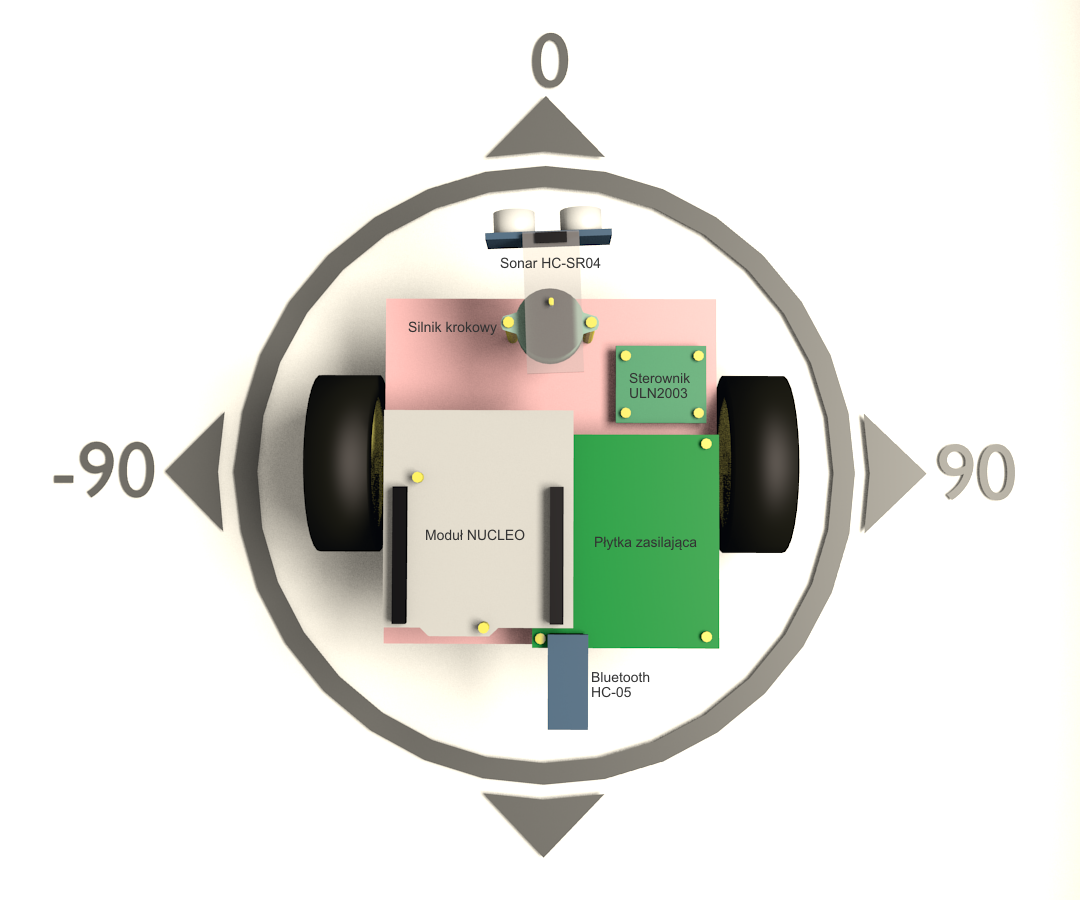
\includegraphics[height=\linewidth,angle=90]{robot4b.png}
\caption{Model 3D robota z zaznaczonym kątem akustycznym}
\label{m3D1}
\end{figure}
\begin{figure}[p]
\centering
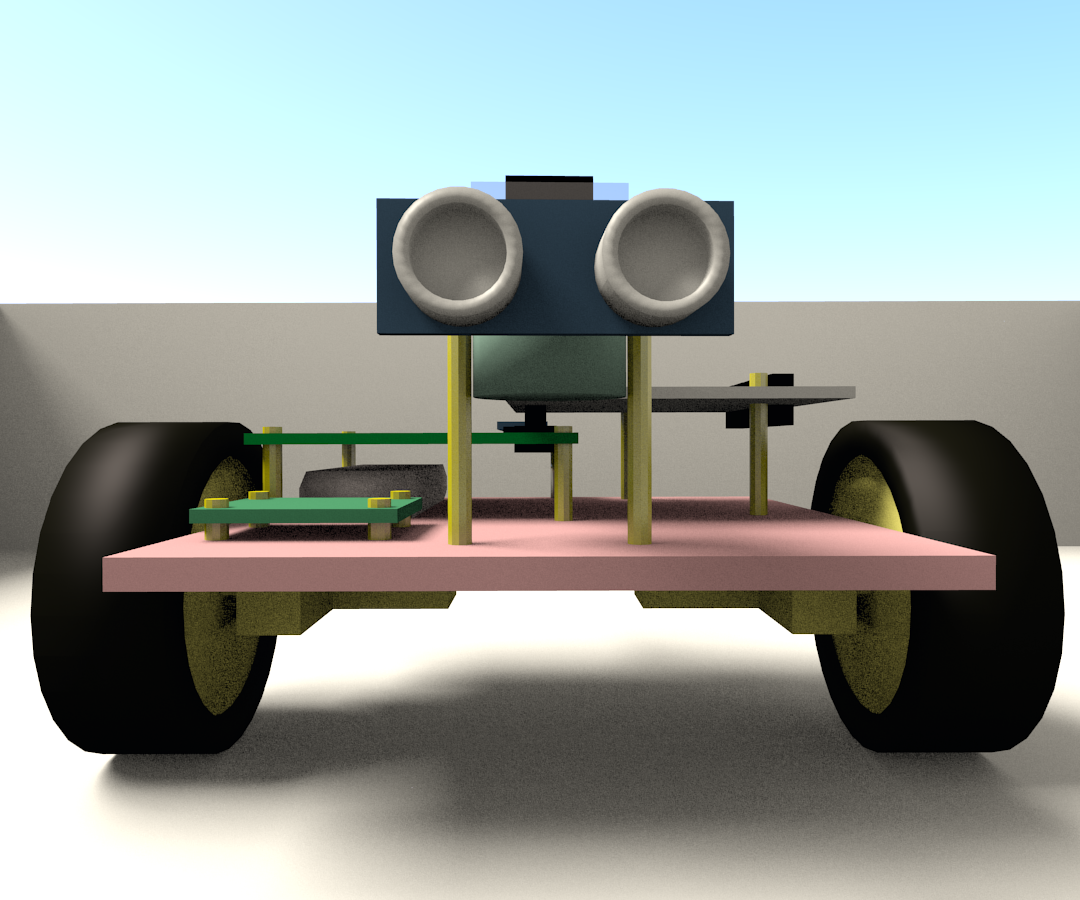
\includegraphics[width=0.8\linewidth]{robot3.png}
\caption{Model 3D robota}
\label{m3D2}
\end{figure}
\begin{figure}[p]
\centering
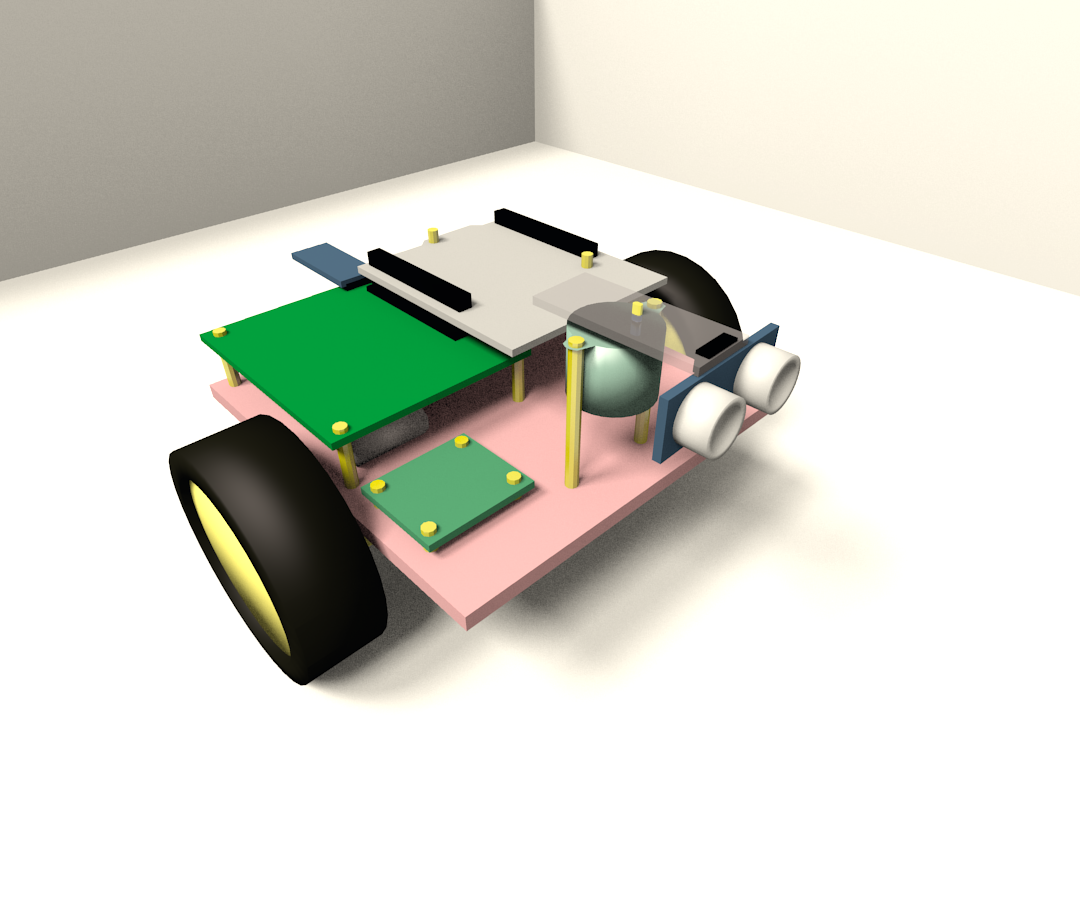
\includegraphics[width=0.8\linewidth]{robot2.png}
\caption{Model 3D robota}
\label{m3D3}
\end{figure}

\subsection{Połączenia elektryczne}
Do zasilenia płytki zastosowaliśmy akumulator li-pol o napięciu 7.4V. Napięcie akumulatora zostało ustabilizowane na dwóch poziomach - 3.3V oraz 5V, ponieważ takie jest wymagane do zasilania poszczególnych modułów. Aby otrzymać takie poziomy zastosowaliśmy stabilizatory napięcia LDO LM1117t (dla 3V3) oraz L7805BV (dla 5V). W celu zabezpieczenia układu zastosowana została dioda prostownicza (zabezpieczenie przed odwrotną polaryzacją) oraz kondensatory (redukcja zakłóceń). \newline
Moduł NUCLEO został zasilony napięciem 5V (pin E5V). \newline
Rysunek \ref{schem1} przedstawia połączenia sekcji zasilania.
\begin{figure}[H]
\centering
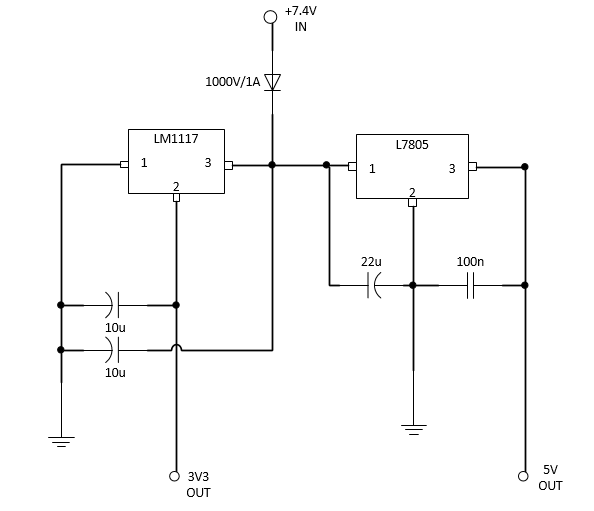
\includegraphics[width=0.8\linewidth]{schem1.png}
\caption{Schemat podłączenia zasilania}
\label{schem1}
\end{figure}
Rysunek \ref{schem2} przedstawia połączenia pinów modułu NUCLEO z pozostałymi modułami.
\begin{figure}[H]
\centering
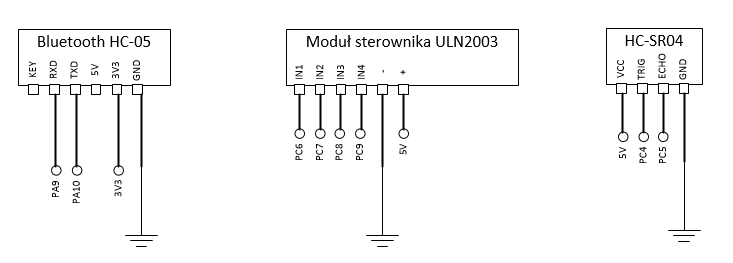
\includegraphics[width=0.8\linewidth]{schem2.png}
\caption{Schemat połączeń modułów}
\label{schem2}
\end{figure}

\subsection{Kosztorys}
Na etapie założeń oszacowaliśmy, że będziemy potrzebowali 311 zł do realizacji projektu. Jak widać na poniższym zestawieniu udało się to zrealizować niższym kosztem. Koszty wzrosłyby gdybyśmy rozpoczęli montaż stelażu. Wtedy należałoby dokupić jeszcze pleksę, słupki montażowe, uchwyty do silników oraz zestawy śrubek. 
\begin{table}[H]
\begin{center}
\begin{tabular}{|c|c|c|}
\hline
\textbf{Element} & \textbf{Cena całkowita(zł)} & \textbf{Zakup poza założeniami}\\ \hline\hline
Zestaw STM32 NUCLEO & 49.56 & \\ \hline
Moduł Bluetooth HC-05 & 31.37 & \\ \hline
Zestaw silników i kół z enkoderami Dagu RS034 & 92.65 & \\ \hline
Silnik krokowy ze sterownikiem ULN2003 & 14.79 & \\ \hline
Kulka podporowa & 9.15 & \\ \hline
Płytka PCB uniwersalna & 3.83 & \\ \hline
Mostek H L298N & 9.28 & \\ \hline
Pozostałe elementy zabezpieczające i zasilające & 4.61 & \\ \hline
Mostek H TB6612 & 11.99 & TAK\\ \hline
Przewody żyłowe & 9.99 & TAK\\ \hline\hline
\textbf{Ogólny koszt:} & 237.22 & \\ \hline
\end{tabular}
\caption{Budżet zadania}
\end{center}
\end{table}

\subsection{Oprogramowanie robota}
Na rysunku \ref{moduly_robota_pc} została przedstawiona komunikacja pomiędzy poszczególnymi modułami robota(zaznaczone na niebiesko). Diagram ten definiuje w jaki sposób wygląda sterowanie robotem oraz komunikacja pomiędzy komputerem osobistym. Widać, że za całe sterowanie jest odpowiedzialny \textit{STM32}. To on powinien decydować jak mają poruszać się silniki, jak powinny być przetworzone informacje z enkoderów oraz czujnika ultradźwiękowego. Ostatecznie to on jest odpowiedzialny za wysyłanie oraz odbieranie informacji i przetwarzanie komend przychodzących z komputera. 
\begin{figure}[H]
\centering
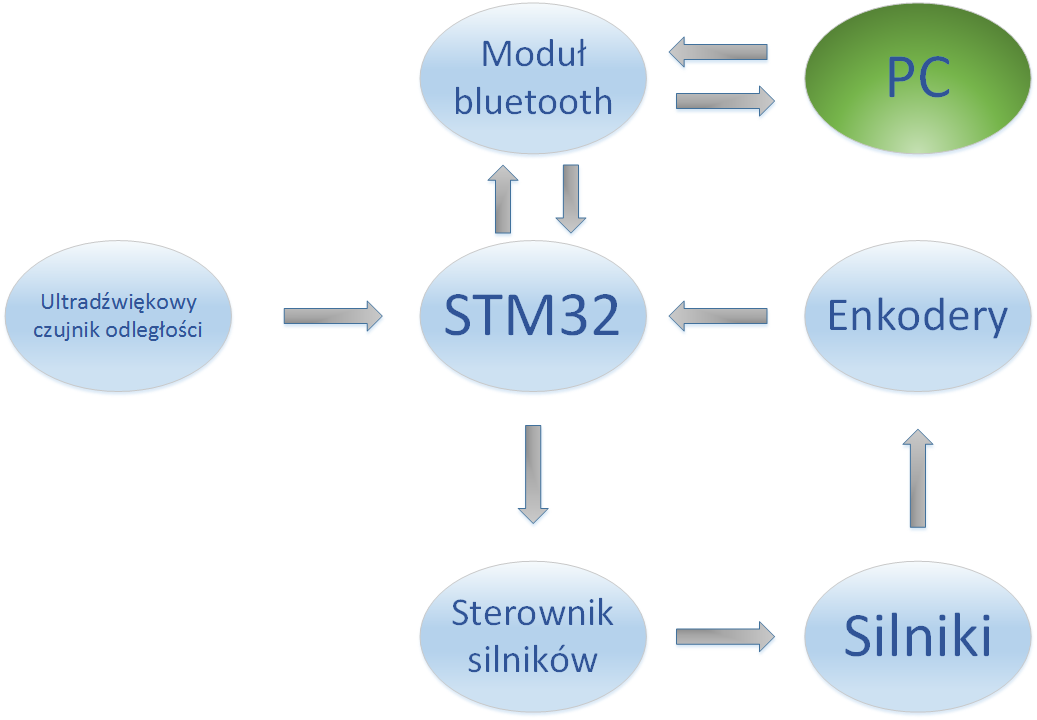
\includegraphics[width=\linewidth]{diagram_komunikacji_modulow_img}
\caption{Diagram przedstawiający moduły robota i PC oraz komunikację pomiędzy nimi}
\label{moduly_robota_pc}
\end{figure}

Oprogramowanie robota zostało napisane przy użyciu środowiska Keil $\mu$Vision 5. W projekcie wyorzystaliśmy bibliotekę standard peripheral library

\subsection{Ostateczny efekt robota}
Ostatecznie połączone zostały ze sobą sekcja zasilania, moduł NUCLEO, silnik krokowy sterowany przy użyciu sterownika ULN2003, moduł Bluetooth HC-05 oraz czujnik ultradźwiękowy HC-SR04. W tej sytuacji robot nie może się sam przemieszczać, ale za to jest w stanie wykonywać skanowanie otoczenia co było tematem naszego projektu. \newline
Rysunek \ref{prac1} pokazuje rzeczywiście połączone moduły.
\begin{figure}[p]
\centering
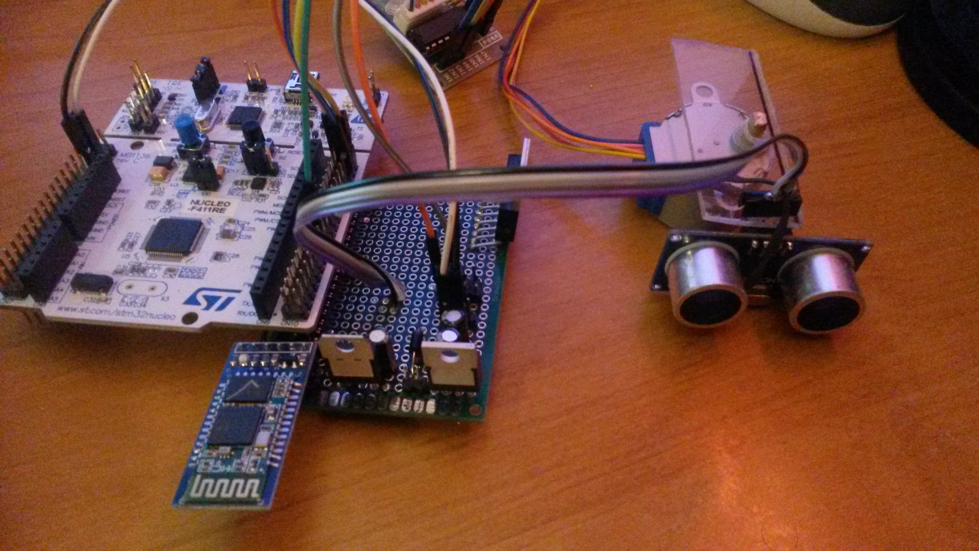
\includegraphics[width=\textheight, angle=90]{prac1.jpg}
\caption{Ostateczny wygląd robota}
\label{prac1}
\end{figure}


\section{Wygląd aplikacji komputerowej}
Główna aplikacja komputerowa składa się z widżetów oraz dodatkowych okien wyświetlanych w przypadku reakcji na błędy lub wywołanie akcji z poziomu paska menu.
\subsection{Widżety dokowane}
Aplikacja składa się z głównego okna widocznego na rysunku \ref{app2}.
\begin{figure}
\centering
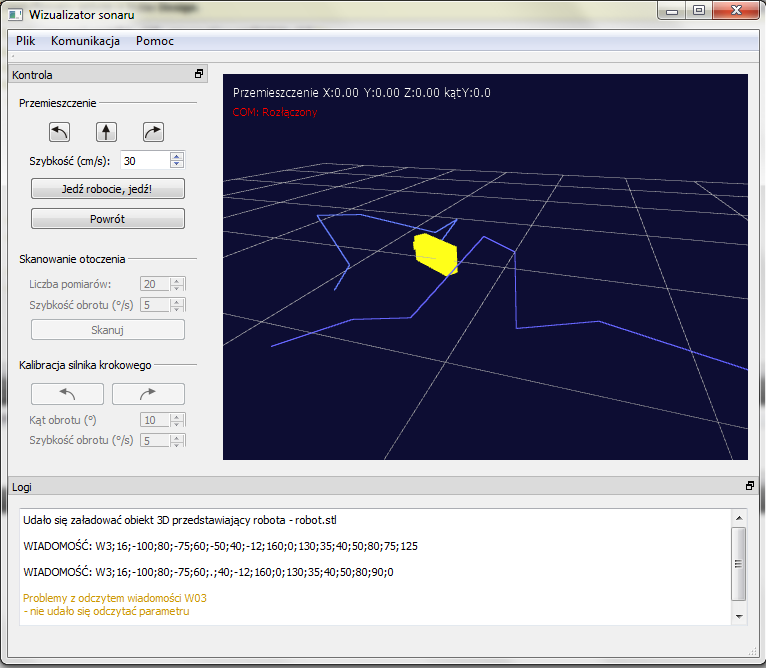
\includegraphics[width=\linewidth]{app2.png}
\caption{Wygląd aplikacji}
\label{app2}
\end{figure}
\begin{figure}[p]
\centering
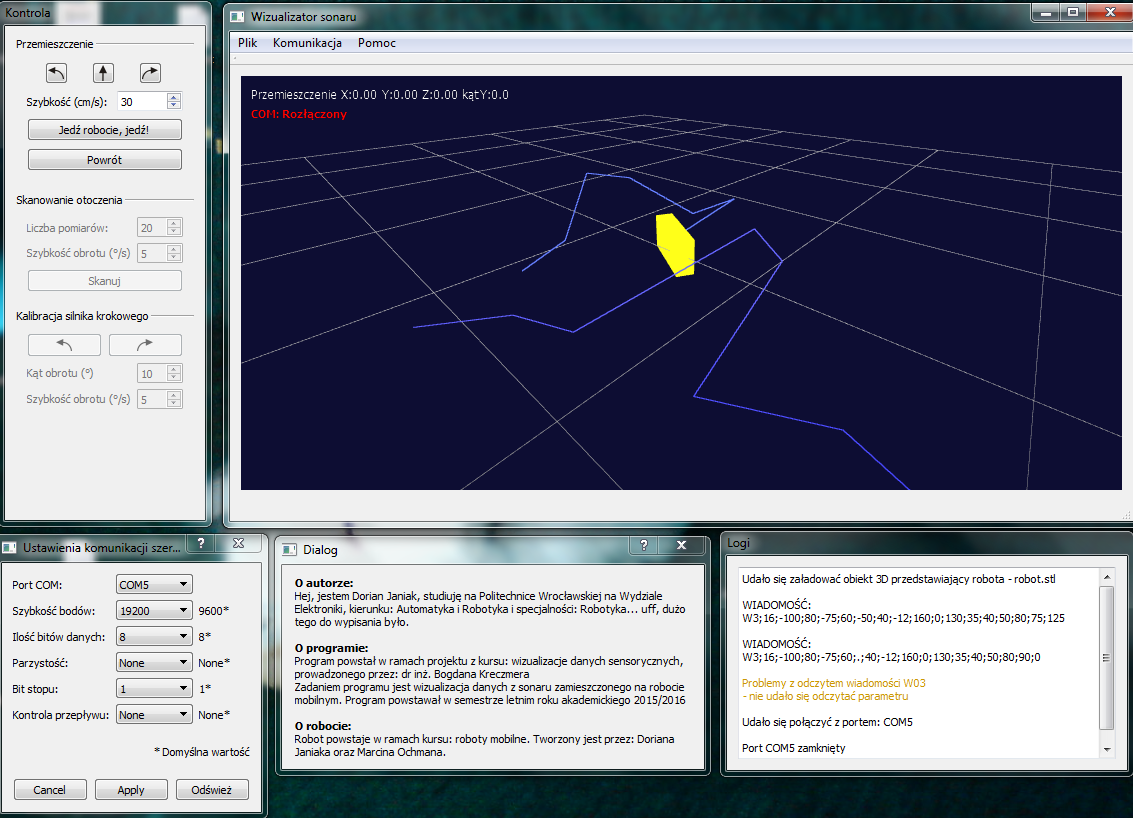
\includegraphics[width=\textheight, angle=90]{app5.png}
\caption{Otwarte kilka okien oraz widżetów - otwieranie na kilku monitorach}
\label{app5}
\end{figure}
W oknie znajdują się trzy widżety: Kontrola, Logi oraz widok 3D. Oba pierwsze widżety są dokowane i mogą zostać odłączone. Pozwala to na wygodniejsze operowanie lub nawet rozkładanie widoku aplikacji na kilka monitorów (rysunek \ref{app5} ). Widżet \textbf{Logi} zawiera jedynie pole tekstowe, którego edytować nie można i w którym pojawiają się wszelkie informacje na temat statusu operacji oraz aplikacji. Zostały wyróżnione różnego typu komunikaty:
\begin{itemize}
\item kolor czarny - zwykła informacja
\item kolor pomarańczowy - ostrzeżenie
\item kolor czerwony - błąd (ale nie krytyczny)
\end{itemize}
Widżet \textbf{Kontrola} składa się z grup:
\begin{itemize}
\item Przemieszczenie - gdzie udostępnione zostały trzy przyciski do sterowania pozycją robota w jakiej chcielibyśmy, aby ostatecznie się znalazł. Aby nakazać robotowi przemieszczenie się do zadanej pozycji należy nacisnąć przycisk \textit{Jedź robocie, jedź!} (Choć należałoby się zastanowić czy przycisk nie powinien nazywać się \textit{Robocie, niech ktoś cię przesunie!} w kontekście niezamontowanych kół do robota). W przeciwnym wypadku robot się nie znajdzie w zadanej pozycji i przy najbliższym skanowaniu otoczenia lub przy naciśnięciu przycisku \textit{Powrót} robot powróci do ostatniej zapamiętanej pozycji (takiej, do której miał dojechać). Można zadać również szybkość jazdy robota. Robot nie musi jej obsłużyć.
\item Skanowanie otoczenia - grupa pozwala na nakazanie robotowi wykonania skanu otoczenia. Skanowanie odbywa się w zakresie 90 do -90 stopni. Można zadać ile pomiarów ma się znaleźć w ramach jednego skanowania i z jaką szybkością ma się wykonywać skanowanie (obrót silnika krokowego). Aby grupa była dostępna aplikacja musi połączyć się z robotem. 
\item Kalibracja silnika krokowego - grupa pozwala na obrócenie silnika krokowego (sterowanie kątem akustycznym czujnika odległościowego) bez wykonywania pomiaru i odczytu mapy otoczenia. Aby grupa była dostępna aplikacja musi połączyć się z robotem.
\end{itemize}

\subsection{Widok 3D}
Główną część okna stanowi \textbf{widok 3D}, w którym przy użyciu myszy komputerowej można sterować kątem kamery (LPM + ruch), jej przybliżeniem (rolka) oraz przemieszczeniem jej centralnego punktu (PPM + ruch). W oknie tym rysowana jest mapa 3D.
 Widok jest renderowany przy użyciu klas \textbf{QOpenGLWidget} (od wersji Qt 5.4 wyparła QGLWidget) oraz \textbf{QOpenGLFunctions}, obsługujących OpenGL. W oknie pojawiają się takie obiekty jak:
\begin{itemize}
\item wyniki skanowania - widoczne na screenie (linie w odcieniach niebieskiego). Każdy dodatkowy pomiar jest podnoszony względem poprzedniego (wzdłuż osi Y) oraz jest rozjaśniany jego kolor. Pozwala to odróżnić kolejne pomiary od siebie. Jest to w szczególności przydatne gdy okaże się, że w trakcie jednego skanowania zostanie zarejestrowany pomiar bardziej odległy niż 3m - wtedy program odrzuca taki pomiar i siatka zostaje rozerwana w tym miejscu. Wtedy mimo kilku osobnych podsiatek można zauważyć, że pochodzą one z tego samego pomiaru, ponieważ są na jednakowej wysokości oraz o jednakowym kolorze.
\item robot - robot jest symbolizowany przez żółty obiekt. W praktyce można jednak obiekt ten zmienić poprzez podmianę pliku \textbf{objects/robot.stl}.
\item siatka - domyślnie jedna kratka odpowiada kwadratowi o boku 1 metru. 
\end{itemize}

\subsection{Dodatkowe okna}
Poważniejsze błędy, wymagające uwagi użytkownika są raportowane okienkiem błędu. 
\begin{figure} [H]
\centering
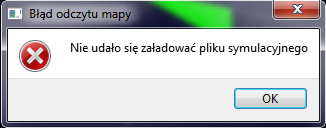
\includegraphics{error_screen.png}
\caption{Komunikat błędu}
\label{error_screen}
\end{figure}
Po wybraniu opcji \textit{Konfiguracja} z menu \textit{Komunikacja} wyświetla poniżej przedstawione okno konfiguracji połączenia szeregowego. 
\begin{figure} [H]
\centering
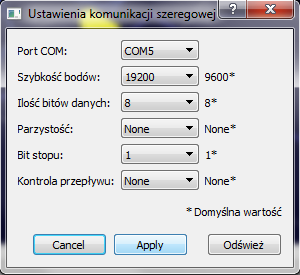
\includegraphics{app3.png}
\caption{Konfiguracja połączenia szeregowego}
\label{app3}
\end{figure}
Po wybraniu opcji \textit{Wyświetl informacje} z menu \textit{Komunikacja} wyświetla się poniższe okno z podsumowaniem aktualnie ustawionych parametrów komunikacji poprzez port szeregowy. 
\begin{figure} [H]
\centering
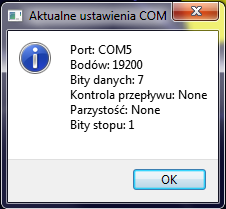
\includegraphics{app6_small.png}
\caption{Aktualnie ustawiona konfiguracja połączenia szeregowego}
\label{app6}
\end{figure}

\subsection{Diagramy}
Poniżej zostały zaprezentowane diagramy klas oraz przypadków użycia dla aplikacji komputerowej.
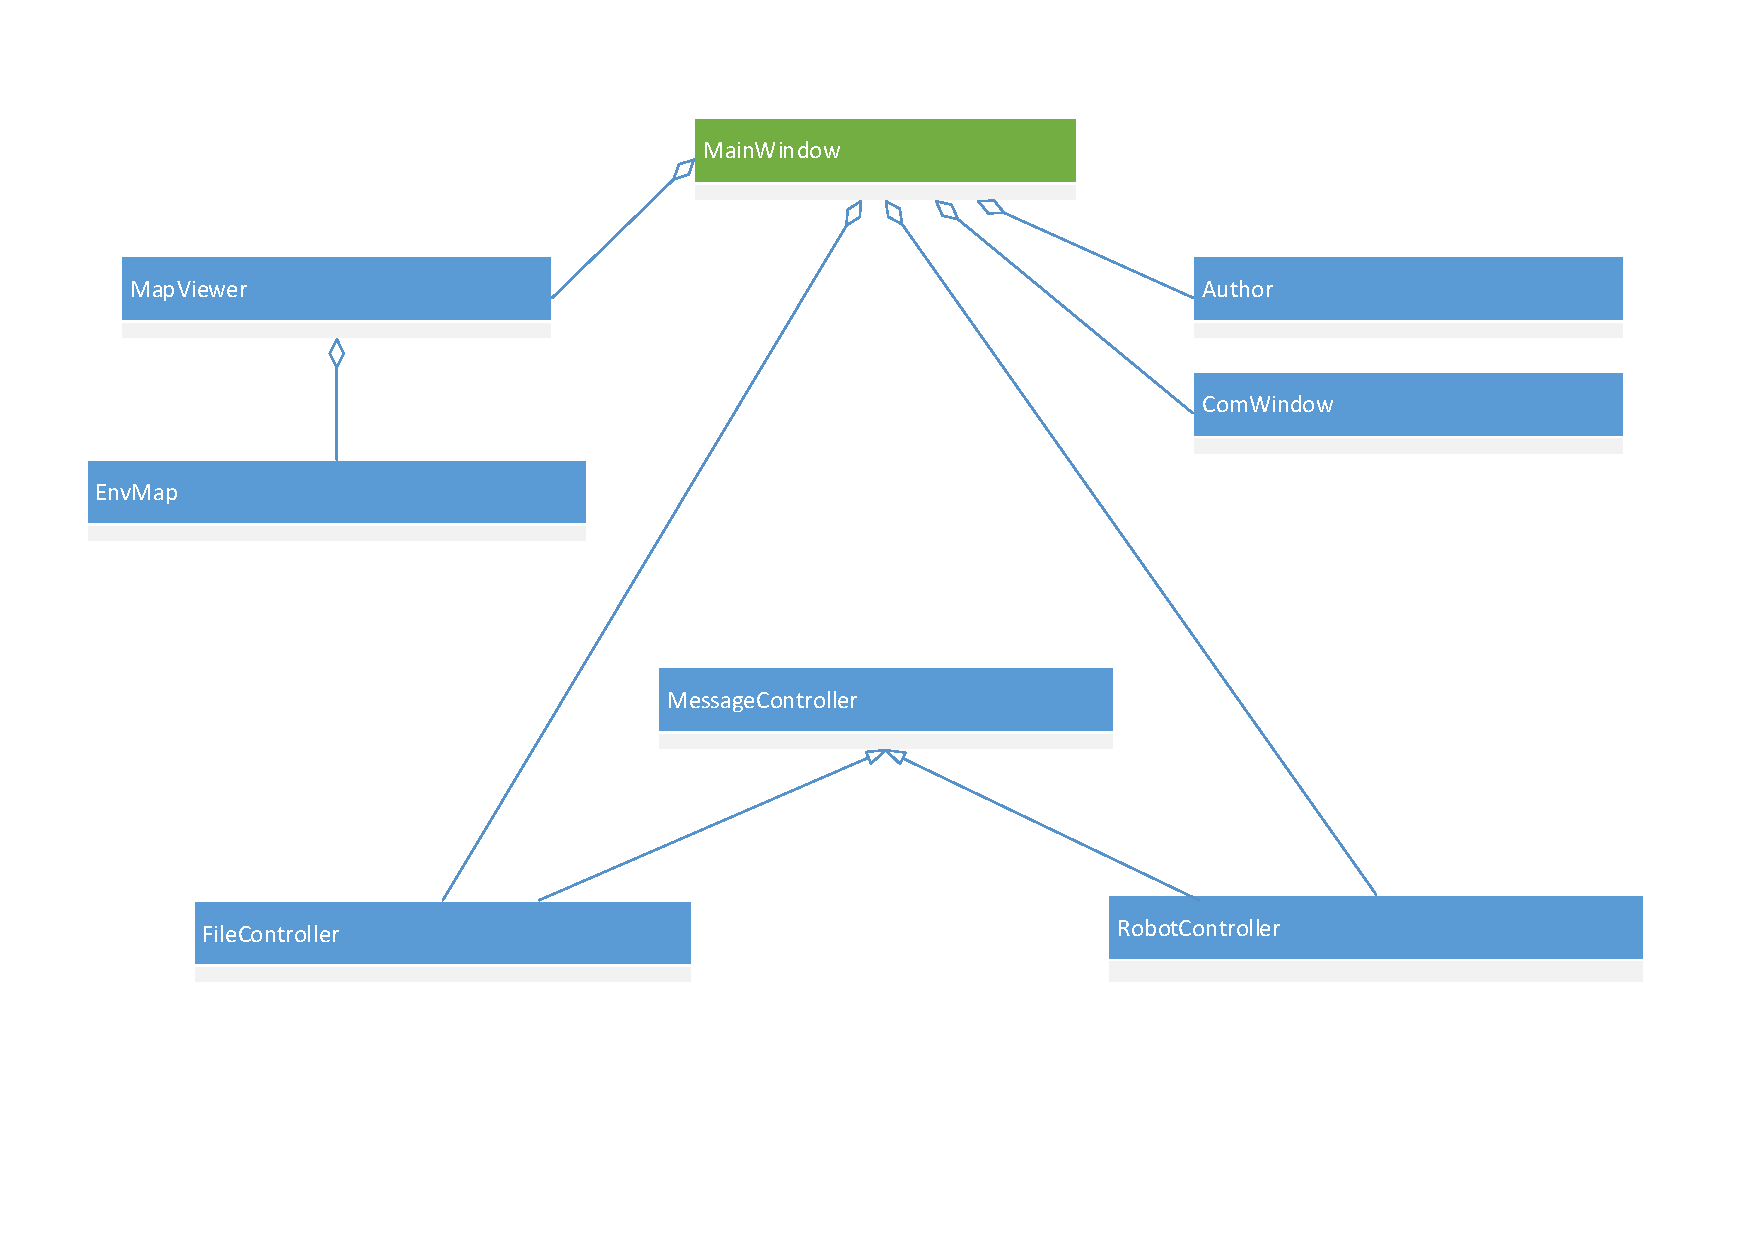
\includepdf[pages={1},landscape=true]{d_klas4.pdf}
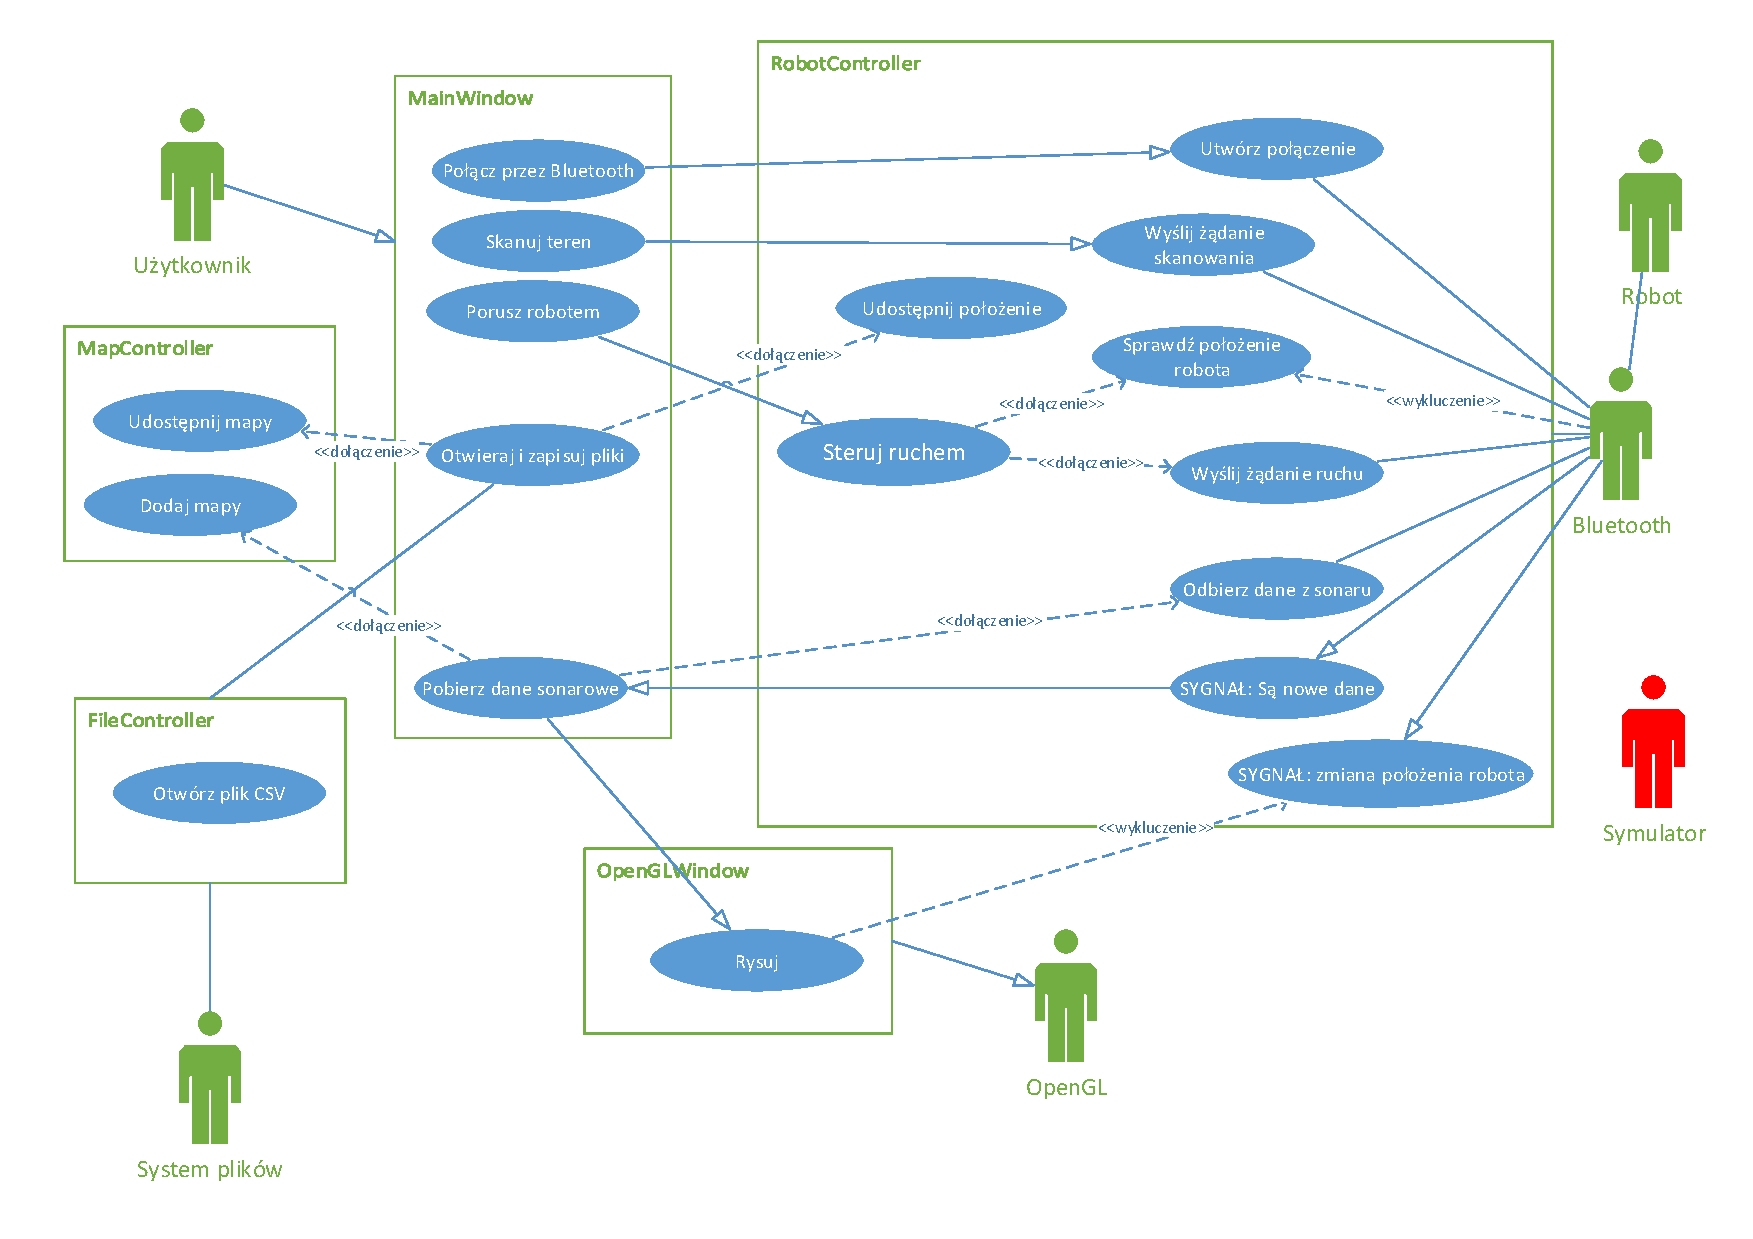
\includepdf[pages={1},landscape=true]{przypadki4.pdf}

\section{Test robota}
W ramach testu przeprowadzone zostało skanowanie mieszkania. Przeskanowane zostały 3 pokoje. Rysunek \ref{stancjac} przedstawia wynik skanowania. Bez znajomości geometrii pomieszczeń trudno wywnioskować jak wygląda pomieszczenie na podstawie samego skanu sonaru. Rysunek \ref{stancjad} przedstawia ten sam wynik skanowania z naniesionymi dodatkowo informacjami nt. geometrii pomieszczeń. Jak widać wynik okazuje się całkiem zbieżny z rzeczywistą geometrią. Należy również zauważyć, że przesuwanie robota mogło nanieść spore błędy na wynik skanu. 
\begin{figure}[p]
\centering
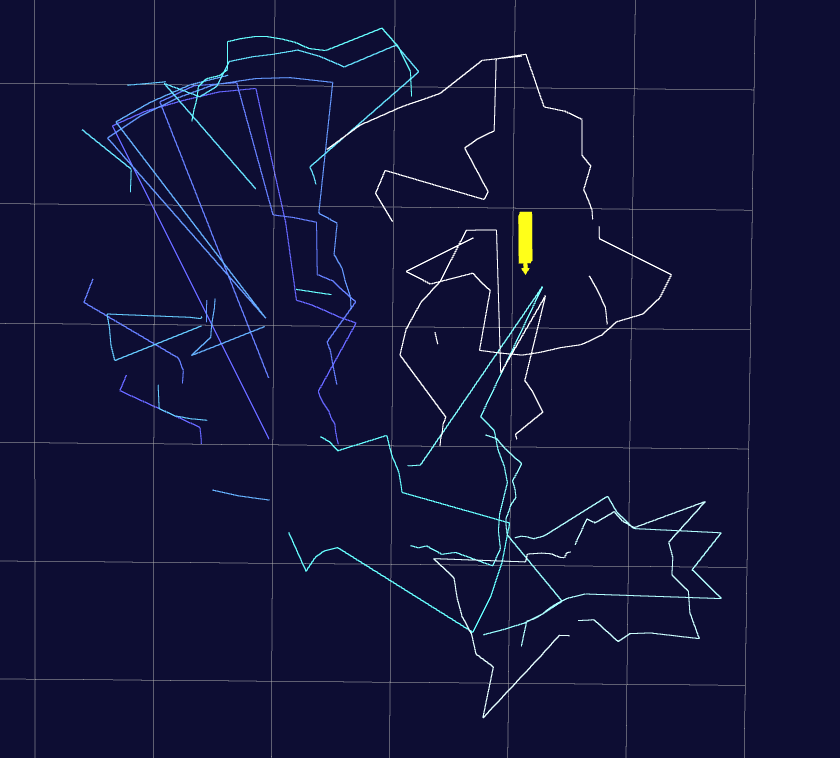
\includegraphics[width=\linewidth]{stancjac.png}
\caption{Wynik skanowania}
\label{stancjac}
\end{figure}
\begin{figure}[p]
\centering
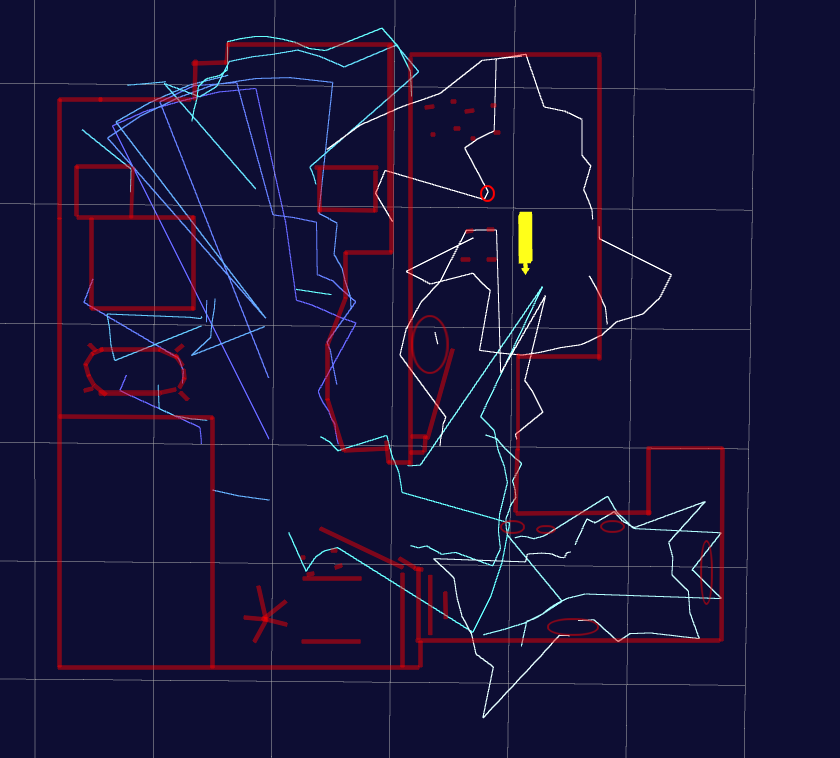
\includegraphics[width=\linewidth]{stancjad.png}
\caption{Wynik skanowania z naniesioną geometrią pomieszczeń}
\label{stancjad}
\end{figure}

\section{Podsumowanie}

Niestety, nie udało nam się w całości zrealizować projektu opisanego w pierwszym dokumencie z założeniami projektowymi. Nie zrealizowaliśmy funkcjonalności poruszania się robota. Przyczyną był źle ułożony harmonogram, który zakładał, że zrobimy znacznie więcej niż byliśmy w stanie wykonać. Praca nad innymi, równie ambitnymi projektami w tym semestrze spowodowała, że prace nad robotem posuwały się niewystarczająco szybko, co spowodowało, że nie byliśmy w stanie zbudować robota na czas. Jesteśmy jednak zadowoleni z wykonanej pracy, ponieważ robot daje możliwość skanowania otoczenia i jego wizualizacji w trybie 3D.

\section{Materiały źródłowe}

Naszym głównym źródłem informacji do stworzenia aplikacji były strony dokumentacji technicznej bibliotek - \textit{Qt5} oraz \textit{OpenGL}. Strony główne zostały zamieszczone poniżej:

\begin{itemize}
\item http://doc.qt.io/qt-5/reference-overview.html
\item https://www.opengl.org/documentation/
\end{itemize}

Natomiast do obsługi modułów robota zosały wykorzystane informacje zawarte pod poniższymi adresami:

\begin{itemize}
\item http://www.mlodedrwale.pl/2013/07/05/tani-modul-bluetooth-cz1/
\item http://www.python.rk.edu.pl/w/p/sterowanie-silnikami-krokowymi-i-serwomechanizmami-za-pomoca-pymcu/
\item http://www.bajdi.com/adding-encoders-to-those-cheap-yellow-motors/
\end{itemize}


\end{document}
